\documentclass[12pt,oneside,a4paper,bibtotoc,liststotoc]{scrreprt}
\usepackage{remreset}

%% Listings
\usepackage{listings}
\lstset{
  basicstyle=\footnotesize, 
  stringstyle=\ttfamily,
  frame=single,
  numberbychapter=false, % Listings vom Anfang bis zum Ende
                         % durchnummerieren
  captionpos=b
}
% Fußnoten, Tabellen und Grafiken von Anfang bis Ende durchnummerieren.
\usepackage{chngcntr}
\counterwithout{footnote}{chapter}
\counterwithout{table}{chapter}
\counterwithout{figure}{chapter}

% Überschriften bis zur dritten Ebene durchnummerieren
\setcounter{secnumdepth}{3}
% Überschriften bis zur zweiten Ebene in den TOC
\setcounter{tocdepth}{2}

%% Typographie-Schnickschnack
\usepackage[T1]{fontenc}
\usepackage{lmodern}
\usepackage{ellipsis} 

%% Absatzformatierung
% \parindent=0cm
\parskip=3mm

% Schönere Zeilenumbrüche
\usepackage{microtype}
\tolerance 1414
\hbadness 1414
\emergencystretch 1.5em
\hfuzz 0.3pt
\vfuzz \hfuzz
\raggedbottom
% Schusterjungen und Hurenkinder unterdrücken
\clubpenalty = 10000 
\widowpenalty = 10000 
\displaywidowpenalty = 10000 
% Schuster- und Hurenfußnoten will auch keiner...
\interfootnotelinepenalty=10000 

\usepackage[utf8]{inputenc}
% Mathematischen Formelsatz erlauben
\usepackage{amsmath}
\usepackage{amssymb}
\usepackage[ngerman]{babel}

%% Wenn ein Index verwendet werden soll, folgendes auskommentieren
% \usepackage{makeidx}
% \makeindex

\usepackage{graphicx}

% Erlaube das Setzen von anderne Zeilenabständen (s.u.)
\usepackage{setspace} 

%% Literaturverzeichnis
\usepackage{jurabib}
\jurabibsetup{
	authorformat=abbrv,
        titleformat={short,commasep},
	commabeforerest,
	see,
%        super, %% Konvertiert alle \cite in \footcite
        square,
%        citefull=first,
}
% Typographischer Schnickschnack für Bibliographie
\renewcommand*{\jbauthorfont}{\textsc}
\renewcommand*{\biblnfont}{\scshape\textbf}
\renewcommand*{\bibfnfont}{\normalfont\textbf}

%% % Abstand vor Kapitelüberschriften: 0 cm (um es Bündig zu setzen, negativen Skip verwenden)
\renewcommand*{\chapterheadstartvskip}{\vspace*{0cm}}
%% % Abstand nach Kapitelüberschriften: 1 Zeile
\renewcommand*{\chapterheadendvskip}{\vspace{1\baselineskip}}

% Referenzen verlinken
\usepackage{hyperref}
\hypersetup{ 
    colorlinks,
    citecolor=black,
    filecolor=black,
    linkcolor=black,
    urlcolor=black 
}

% Grad-Zeichen definieren
\newcommand{\grad}{\mbox{\(\mathsurround=0pt{}^\circ\)}}
% (r)-Zeichen definieren
\def\TReg{\textsuperscript{\textregistered}}
% z.B., d.h. usw. Typographisch korrekt setzen
\usepackage{xspace}
\newcommand{\zB}{\mbox{z.\,B.}\xspace}
\newcommand{\dH}{\mbox{d.\,h.}\xspace}
\newcommand{\ua}{\mbox{u.\,a.}\xspace}
\newcommand{\so}{\mbox{s.\,o.}\xspace}
\newcommand{\MSc}{\mbox{M.\,Sc.}\xspace}
\newcommand{\BSc}{\mbox{B.\,Sc.}\xspace}


%% Schönere Tabellen
\usepackage{booktabs}
\usepackage{tabularx}

%% Ränder setzen
\usepackage[left=5cm,right=3cm,top=1.5cm,bottom=2cm,includeheadfoot]{geometry}

%% Abkürzungsverzeichnis
\usepackage[printonlyused]{acronym}

%% Allow really fixed positions for Tables
\usepackage{float}
\restylefloat{table}

%% Gedrehte Tabellen
\usepackage{rotating}

%% Trennung tweaken: Manche Wörter will man ggf. anders trennen als
%% der Algorithmus das vorsieht oder ggf. auch garnicht
\hyphenation{Java-Script}
\hyphenation{Cookies}

\begin{document}
\begin{titlepage} 
\begin{figure}[H]
  \begin{flushright}
    
\includegraphics{img/fh-koeln-logo.png}
    \label{logo_fh_köln}
  \end{flushright}
\end{figure}

\begin{center}
\textbf{\Large\newline  Fachhochschule Köln\\
Cologne University of Applied Sciences\\[0.1cm]
\normalsize Campus Gummersbach\\
Fakultät für Informatik und Ingenieurwissenschaften\\[0.5cm]}

 
\Large Verbundstudiengang Wirtschaftsinformatik\\[0.5cm]

\large Masterthesis\\[0.1cm]
  
% Title
{ \huge \bfseries \ Konzepte der Nebenläufigkeit  \\[0.1cm]
        unter Android \\[0.5cm]
        
}
\vfill

\begin{table}[h]
\centering
\begin{tabular}{ll}
  Prüfer:         & Prof. Dr. Erich Ehses \\
  Zeitprüfer:     & Prof. Dr. Frank Victor \\
  vorgelegt am:   & \today \\
  von cand.:      & Stephan Wagner \\
  aus:            & Overath \\
  Telefon-Nr.:    & +49-176-80007570 \\
  Matrikel-Nr.:   & 1106011828 \\
  E-Mail-Adresse: & stephan.wagner.mi738@gmail.com
\end{tabular}
\end{table}
\end{center}
\end{titlepage}



\onehalfspacing % 1,5-facher Zeilenabstand

\chapter*{Zusammenfassung}
Diese Thesis behandelt das Thema „Konzepte der Nebenläufigkeit unter Android“. Darin wird zunächst als Einführung in die Thematik, die Nebenläufigkeit allgemein mit ihren unterschiedlichen Ausprägungen (Prozess-/Threadebene) erläutert und die Risiken die mit Nebenläufigkeit einhergeht skizziert. Dabei ist ein besonders wichtiger Punkt der Botschaftenaustausch, der mittels unterschiedlicher Techniken realisierbar ist. Auch hier birgt jede Technologie ihre individuellen Vor- und Nachteile.
Die Nebenläufigkeit unter Android unterliegt einigen Besonderheiten, die sich teilweise aus den Restriktionen des Betriebssystems ergeben, aber auch aus den Anforderungen für die Android Applikationsentwicklung, die der StyleGuide vorgibt. So ist die grundsätzliche Anforderung, dass Applikationen ansprechbar bleiben. Eine Applikation, insbesondere eine Gui Applikation sollte somit beim Start von Operationen weder blockieren oder nicht mehr auf Benutzereingaben reagieren. Technisch bedeutet dies, dass zeitaufwändige Operationen nie auf dem Main Thread der Applikation stattfinden dürfen. Stattdessen müssen derartige Operationen in Hintergrundthreads ausgelagert werden. Im Kapitel 2 werden hierzu drei unterschiedliche Konzepte an Hand konkreten Beispielimplementierungen vorgestellt und in der jeweiligen Funktionsweise analysiert.
\begin{itemize}
\item Java Concurrency nach Java SE
\item Android Concurrency aus dem Android SDK
\item RXJava Framework
\end{itemize}
Die aus der technischen Analyse gewonnenen Erkenntnisse werden in Kapitel 3 genutzt um Chancen und Risiken der einzelnen Konzepte zu diskutieren. Um die Ergebnisse aus dem Diskurs für zukünftige Entscheidungsfindungen zu Rate ziehen zu können fließen die aus der Detailanalyse gewonnenen Ergebnisse in eine Szenarien basierte Analyse ein, um daraus Anhaltspunkte für den sinnvollen Einsatz der Konzepte abzuleiten.

\tableofcontents
\listoffigures


\chapter{Einleitung}
\section{Motivation}
Mobile Endgeräte begleiten immer mehr Menschen in ihrem Alltag. Damit einher geht die intensive Nutzung von sog. Apps., womit Applikationen auf den mobilen Endgeräten bezeichnet werden. Mit der zunehmenden Leistungsfähigkeit der Geräte werden auch immer komplexere Applikationen realisierbar. Wurde zu den Anfängen der Applikationsentwicklung für mobile Endgeräte lediglich einfache Funktionalität in Applikationen integriert, werden heute mit unter teilweise sehr rechenintensive und komplexe Funktionalitäten entwickelt. Eine optimale Konzeption der Aufgabenverarbeitung innerhalb der Applikation kann dabei einen entscheidenden Faktor für die Performance und damit auch die Akzeptanz beim Nutzer darstellen. Damit gewinnt die Nebenläufigkeit auch in der Applikationsentwicklung für mobile Endgeräte an Wichtigkeit. Nebenläufigkeit oder auch Parallelverarbeitung bezeichnet in der Informatik die Eigenschaft eines Programms oder eines Systems verschiedene Aufgaben zeitgleich, also parallel zu bearbeiten. Die jeweilige Verarbeitung kann dabei in sich abgeschlossen sein, d.h. die zu verarbeitenden Aufgaben sind voneinander unabhängig, oder die Verarbeitung hängt von den Ergebnissen aus anderen Aufgaben ab. Je nach Art und Weise der Parallelverarbeitung sind verschiedene Problematiken und Risiken zu beachten. Für Nebenläufigkeit unter dem Android Betriebssystem sind zusätzliche Besonderheiten zu beachten. Dieses Betriebssystem ist auf mobile Endgeräte zugeschnitten und hat diesbezüglich spezielle Anforderungen an Applikationen die darauf laufen sollen. Die Firma Google als Hersteller vom Betriebssystem Android legt hierbei großen Wert auf die Einhaltung eines StyleGuides der die Benutzbarkeit applikationsübergreifend in einem einheitlichen Standard definiert. Darin wird die grundlegende Anforderung nach der kontinuierlichen Ansprechbarkeit von Applikationen gefordert. Die Frage ist wie kann den Anforderungen an Android Applikationen mittels unterschiedlicher Konzepte der Nebenläufigkeit begegnet werden, sodass das von Google geforderte Ziel der Ansprechbarkeit erreicht werden kann. Welche Problemstellungen, Restriktionen oder Risiken gehen mit der Verwendung bestimmter Konzepte einher und wie praktikabel sind diese für den konkreten Praxiseinsatz? 

\section{Zielsetzung und Vorgehen}
In dieser Arbeit soll untersucht werden, wie konkurrierende Parallelverarbeitung in mobilen Anwendungen realisiert werden kann. Dabei besteht das Ziel, die Entwicklung von Nebenläufigkeit durch Verwendung unterschiedlicher Techniken zu vereinfachen und ggf. auf einem höheren Abstraktionsniveau ab zu bilden. Zunächst gilt es in einer kurzen Einführung in die Thematik, die grundsätzlichen Definitionen kurz zu erläutern und auf Besonderheiten der Parallelverarbeitung unter Android einzugehen. Weiter wird ein Überblick über eine Auswahl von unterschiedlichen Konzepten der Nebenläufigkeit unter Android erarbeitet. Diese werden mittels einfacher Beispiele vorgestellt und analysiert. Den Abschluss bildet ein kritischer Diskurs, um in Abhängigkeit vom Einsatzkontext eine Differenzierte Sicht auf die Anwendung der einzelnen Konzepte zu erhalten. Die Ergebnisse des Diskurses werden in einer szenarienbasierten Analyse aufgegriffen um diese greifbarer zu machen.

\section{Begriffsdefinition und Grundlagen der Nebenläufigkeit}
Um sich den Konzepten der Nebenläufigkeit anzunähern, werden zunächst einige Begriffsdefinitionen benötigt. Die Nebenläufigkeit meint dabei konkret die parallele Verarbeitung von Aufgaben. Hierzu wird eine Aufgabe in Unteraufgaben aufgeteilt, um diese  weitestgehend von einander unabhängig abzuarbeiten. Die Definition wie diese Verarbeitung ablaufen soll, ist in einem Programm hinterlegt. Die Ausführung von Programmen wird von Prozessen und Threads geregelt. Diese werden im folgenden Abschnitt definiert und ein tieferes Verständnis von der Parallelverarbeitung auf Betriebssystemebene erarbeitet.

\section{Prozesse und Threads}
Die genauen Eigenschaften von Prozessen und Threads sind abhängig vom Betriebssystem auf dem sie laufen. Da in dieser Arbeit der Fokus auf Nebenläufigkeit unter Android liegt, beziehen sich die folgenden Erläuterungen zu Prozessen und Threads auf das allgemeine Unix/Linux Betriebssystem auf dem Android basiert.

\subsection{Prozess}
Wird eine Anwendung gestartet, so erzeugt das Betriebssystem zunächst einen Prozess, der den Adressraum für sämtliche Programmdaten und Komponenten reserviert. Für Prozesse kann folgende Definition getroffen werden. Sie gilt betriebssystemübergreifend:
\begin{center}
Ein Prozess stellt ein Programm in Ausführung dar und
ist für die Kontrolle(Sicherung) der damit verbundenen Betriebsmittel
verantwortlich.
\end{center}
Die Prozesse sind (in der Regel) an einen Benutzer gebunden, welcher wiederum über bestimme Rechte u.a. im Dateisystem verfügt. Dabei sind für Linux Betriebssysteme folgende Prinzipien zu beachten:
\begin{itemize}
\item Hierarschische Prinzip
\item Sandbox Prinzip
\end{itemize}
Das hierarchische Prinzip schreibt die Abhängigkeit von Prozessen gegenüber ihren Erzeugern vor. Mit Ausnahme des Root Prozesses des Betriebssystems, werden alle Anwendungen durch einen Vater Prozess erzeugt. Die damit verbundene Vater-Kind Abhängigkeit bildet eine Baumstruktur, in der jeder Prozess seinen erzeugenden Prozess kennt. Ein Prozess kann nur aus anderen Prozessen heraus erzeugt werden. Stirbt ein Prozess, so werden die Kind Prozesse in der Regel vom Root Prozess des Betriebsystems adoptiert.\newline
Das Sandbox Prinzip ist ein Sicherheitskonzept aus dem Kern eines Linux/Unix Betriebssystems. Darin wird sichergestellt, dass jede Anwendung nur die eigenen Daten sehen darf. So wird bei der Installation für jede Anwendung ein eigener Betriebssystem- User erzeugt, der über spezielle Rechte zu Prozessen und Dateien verfügt. Damit wird zum Ausführungszeitpunkt verhindert, dass Programmdaten für andere Programme sichtbar werden. Die Sicht jedes Prozesses einer Anwendung ist begrenzt auf die Ressourcen die dem jeweiligen Betriebssystem User zugeordnet sind.

\subsection{Thread}
Die Begriffe Prozesse und Threads dürfen nicht synonym verwendet werden. So kann ein Thread wie folgend Definiert werden:
\begin{center}
Ein Thread stellt einen Ausführungsfaden
eines Programmes dar.
\end{center}
Dieser besteht aus aus einem aktuellen Befehlszeiger, einem eigenen Stack und dem Inhalt der Prozessorregister. Zum Start einer Anwendung wird der sog. Main Thread erzeugt. Aus diesem lassen sich beliebig weitere Threads erzeugen. Dabei besteht keine hierarchische Bindung wie bei der Vater-Sohn Prozesshierarchie. Innerhalb eines Prozesses erzeugte Threads erhalten Zugriff auf den hier reservierten Speicher des Prozesses. Alle in einem Prozess erzeugte Threads sind von diesem abhängig. Wird demnach ein Prozess terminiert, so werden auch alle darin erzeugte Threads terminiert.

\section{Botschaftenaustausch und Kommunikation}
Der Botschaftenaustausch zwischen Prozessen unterscheidet sich vom Botschaftenaustausch zwischen Threads. Während bei der Inter Prozess Kommunikation maßgeblich das Betriebssystem am Austausch von Nachrichten zwischen Prozessen beteiligt ist, können bei der Inter Thread Kommunikation unterschiedliche Techniken unabhängig vom Betriebssystem angewandt werden. Für die Kommunikation zwischen Threads eignen sich z.B. Dateien aber auch sogenannte MessageQueues mit denen Produzenten und Konsumenten Konstrukte erzeugt werden können. Die Inter Thread Kommunikation bleibt begrenzt auf die Threads innerhalb einer Anwendung. Die Inter Prozess Kommunikation dagegen, definiert die Kommunikation über Programm- und Systemgrenzen hinaus. Innerhalb eines Betriebssystems wird in der Regel der Speicherbereich jedes Prozesses in sich gekapselt und vor anderen Prozessen verborgen (s.o. Sandbox-Prinzip). Daher werden Mechanismen seitens des Betriebssystems benötigt (Botschaftenaustausch über Socket, etc..) um die Kommunikation zu gewährleisten. Diese Mechanismen sind aufwendig und eignen sich dadurch weniger für eine effiziente Parallelverarbeitung. Daher konzentriert sich diese Arbeit auf die Kommunikation auf Thread Ebene, und die Inter Prozess Kommunikation wird nicht weiter thematisiert. Die folgenden Abschnitte geben einen Einblick auf gängige Techniken zur Realisierung von Inter Thread Kommunikation.

\subsection{Geteilte Datei/ Speicher}
Einer der einfachsten technischen Mittel für den Daten- /Botschaftenaustauch ist die Nutzung einer gemeinsamen Datei im Dateisystem des Betriebssystems. Dadurch, dass das Betriebssystem den exklusiven Zugriff auf Dateien gewährleisten kann, ist es möglich ohne großen Aufwand eine synchronisierte Kommunikation zu realisieren. Etwas komplexer ist es für die Kommunikation einen Speicherbereich zu allokieren und die Referenz darauf den jeweiligen Kommunikationspartern für den Datenaustausch zur Verfügung zu stellen. In diesem Fall muss der exklusive Ausschluss selbst realisiert werden, falls er gewünscht ist. Hierzu dienen einfache Primitive aus dem java.lang.concurrency Packet.

\subsection{MessageQueues}
Die folgende Abbildung gibt einen schematischen Überblick über die Nutzung einer MessageQueue für die Kommunikation zwischen Objektinstanzen aus unterschiedlichen Threads. Beide Objekt Instanzen müssen eine Referenz auf das MessageQueue Objekt halten um Nachrichten (z.B. Message to Thread B) in diese Queue einzustellen oder herauszuholen. Das Konzept des nachrichtengetriebenen Datenaustausches hat den Vorteil, dass jede Nachricht eine atomare (in sich geschlossene) Einheit darstellt. Dadurch lassen sich einzelne Arbeitsaufträge unterscheiden. Je nach Implementierung der MessageQueue sind auch keine weiteren Synchronisationen mehr nötig.
\begin{figure}[H]
  \begin{centering}
    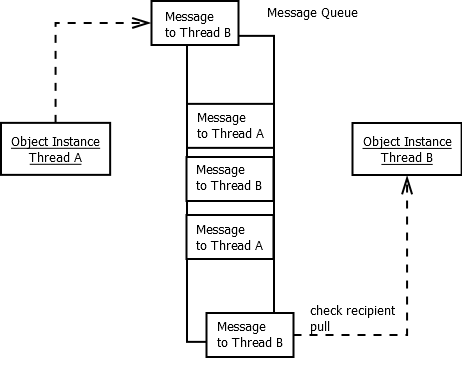
\includegraphics[width=0.8\textwidth]{img/MessageQueue.png}
  %  \caption{MessageQueue}
    \label{MessageQueue}
  \end{centering}
\end{figure}
Die Kommunikation mittels einer MessageQueue kann in zwei Formen realisiert werden:
\begin{itemize}
\item Unidirektional
\item Bidirektional
\end{itemize}
Bei der unidirektionalen Kommunikationsform darf ein Kommunikationspartner nur entweder Nachrichten aus der Queue entnehmen oder hinein geben. In unserem Beispiel dürfte demnach nur die Objekt Instanz des Thread A Nachrichten in die Queue geben und die Objekt Instanz des Thread B darf lediglich aus dieser lesen.\newline
Bei der bidirektionalen Kommunikationsform dürfen beide Kommunikationspartner je Nachrichten in die MessageQueue einstellen wie auch herausnehmen.\newline 
\newline

Die letzten beiden Abschnitte haben einen Überblick über Technologieen gegeben, mit denen der Austausch von Informationen innerhalb einer nebenläufigen Verarbeitung über Thread Grenzen hinaus realisiert werden kann. Dabei stellen MessageQueues eine Abstraktionsebene zur Kommunikation über fest definierten Speicher dar. Die Entwicklung von Nebenläufigkeit kann jedoch auch zu schwerwiegenden Problemen führen.


\section{Risiken von Nebenläufigkeit}
Der Botschaftenaustausch zwischen Threads, sowie deren Synchronisation kann zu schwerwiegenden Problemen im Zuge der Prallelverarbeitung führen. Folgende Szenarien sind eher allgemein gehalten, jedoch gilt es, besonders in dem Kapitel 2  zu den konkreten Implementierungen von Nebenläufigkeit, diese Problematiken zu beachten. In Kapitel 3 werden die in Kapitel 2 zu diskutierenden Beispielimplementierungen u.a. an Hand der hier aufgeführten Risikoszenarien und dem damit verbundenen Fehlerpotential bewertet.


\subsection{Philosophenproblem}
Ein zentrales Problem der theoretischen Informatik ist das Philosophenproblem das erstmals beschrieben wurde durch Edsger W. Dijkstra. Darin wird ein Szenario berschrieben, in dem eine bestimmte Anzahl von Philosophen auf begrenzte Ressourcen zugreifen und bei gleichzeitigem Zugriff sich gegenseitig blockieren können.

\begin{figure}[H]
  \begin{centering}
    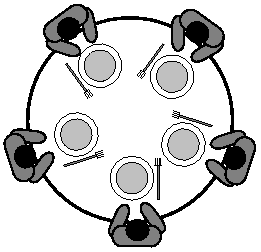
\includegraphics[width=0.6\textwidth]{img/PhilosophenProblem.png}
    \caption{Philosophenproblem \cite[vgl. ]{002}}
    \label{Philosophenproblem}
  \end{centering}
\end{figure}
Die Abbildung zeigt wie eine Gruppe von Philosophen an einem Runden Tisch sitzen, vor ihnen etwas zu Essen. Um zu essen, benötigen nach diesem theoretischen Aufbau die Philosophen die rechte und die linke Gabel neben dem jeweiligen Teller. Dabei versuchen die Philosophen zu nächst die Gabel zu ihrer Linken zu nehmen. Ist die Gabel frei, so behälten sie diese in der Hand bis auch die Gabel auf der rechten aufgenommen werden kann. Kann ein Philosoph eine Gabel zur Zeit nicht nehmen, da sie in Verwendung ist, verweilt er denkend bis die benötigte Gabel frei ist. Versuchen jedoch alle Philosophen gleichzeitig die Gabeln aufzunehmen, so besteht die Gefahr einer Verklemmung (engl. Deadlock). Der Ablauf stockt und die Philosophen verharren denkend bis sie verhungern. In Bezug auf die Kommunikation über geteilten Speicher oder Dateien kann dieses Problem auftreten wenn parallele Zugriffe auf exklusive Ressourcen nicht sauber synchronisiert werden.



\subsection{Race Conditions}
Ein weiteres Problem bei der Parallelverarbeitung tritt bei geteilten Speicher bzw. Daten auf. Folgende Abbildung illustriert das Szenario, dass drei Threads auf einen gemeinsamen Speicherbereich zugreifen. Die Threads eins bis drei greifen konkurrierend lesend, wie schreibend auf den Speicherbereich zu und tauschen darüber Informationen untereinander aus. Der Zugriff erfolgt nach dem Prinzip \glqq Wer zuerst kommt mahlt zuerst\grqq  ( = Race Condition).

\begin{figure}[H]
  \begin{centering}
    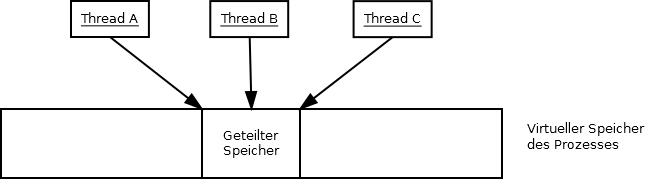
\includegraphics[width=0.8\textwidth]{img/SharedMemory_RaceCondition.png}
 %   \caption{Race_Condition beim Shared Memory  \cite[vgl. ]{002}}
    \label{SharedMemory_RaceCondition}
  \end{centering}
\end{figure}
Ist der Zugriff der Threads auf den Speicher nicht synchronisiert, so kommt es zu dem Shared Memory Effekt, (geteilter Speicher Effekt) nach dem eine Datenstruktur die, die Grundlage von Berechnungen darstellt, durch einen anderen Thread verändert wird, ohne dass die Änderung dem ersten Thread bekannt gemacht wird. Da solche Probleme von der jeweils in diesem Moment vorliegenden Prozessauslastung im System abhängen (tatsächlich gleichzeitig laufende Threads im Multi Core System), sind derartige Effekte schwer reproduzierbar und somit auch die Ursachen schwer zu finden.





\subsection{Speicherleck}
Speicherlecks (eng. Memory Leaks) entstehen häufig aus Programmierfehler heraus, in denen Speicher reserviert, aber dieser nicht mehr freigegeben wird. Geschieht dies ausreichend oft während einer Laufzeit innerhalb des Addressraums des Programmes, so gerät im schlimmsten Fall der seitens der Hardware begrenzte Speicher an seine Grenzen. Das Betriebssystem registriert dieses Verhalten und terminiert sofort die Ausführung des Programmes. Bei der Technik des geteilten Speichers, ist das Risiko eines Speicherlecks z.B. dann präsent, wenn sich der Entwickler um korrekte Dereferenzierung des Speichers und dessen Freigabe explizit kümmern muss. Wird Speicher n-Fach allokiert und nicht wieder freigegeben, so handelt es sich um ein ernstes Speicherleck. Auch bei der MessageQueue sind Speicherlecks möglich, z.B. wenn kontinuierlich Botschaften in die Queue gepackt werden, diese aber nicht aus der Queue wieder herausgenommen werden.

\subsection{Reihenfolgeproblem}
Im Falle einer bidirektionalen Kommunikation mittels einer MessageQueue muss beachtet werden, dass es nicht vorhersehbar ist, in welcher Reihenfolge die Nachrichten in die MessageQueue gelegt werden, oder wann sich welcher Thread eine Message aus der Queue holt. Dies kann zu unerwarteten Verhalten führen. So kann ein Thread B ungewollt blockieren, wenn er für seine weitere Verarbeitung eine bestimmte Nachricht benötigt und diese jedoch sich in der Reihenfolge hinter einer Nachricht für den anderen Thread A befindet. So muss Thread B solange warten bis Thread A seine Nachricht aus der Queue nimmt.
\newline
Welche Konzepte es gibt, um sich den allgemeinen Problematiken und Risiken von Nebenläufigkeit speziell für Android Applikationen zu nähern ist zentraler Forschungsschwerpunkt dieser Arbeit. Diese Konzepte werden im Kapitel 2 im einzelnen vorgestellt.


\section{Parallelverarbeitung und Besonderheiten unter Android}
Im vorangegangenen Abschnitt wurde allgemein auf die Terminologie, die Eigenschaften, sowie die Kommunikation innerhalb von Nebenläufigkeit eingegangen. Hier gilt es nun einen Fokus auf Nebenläufigkeit im mobilen Umfeld zu setzen, insbesondere unter dem Betriebsystem Android. Weiter wird ein erster Einblick in das Komponentenmodell, sowie in den Lebenszyklus von Android Applikationen erarbeitet.


\subsection{Prozesse und Threads unter Android}
\paragraph{Prozess Charakteristika}
Das Android Betriebssystem basiert auf dem Linux/Unix System. Daher gelten die o.g. Eigenschaften zu Prozessen unter dem Linux/Unix Betriebssystem auch für Android. Sie werden lediglich um folgende Charakteristika erweitert.
\begin{enumerate}
\item Fordergrundprozess $\rightarrow$ Fordergrundprozesse sind verantwortlich für alle Komponenten einer Anwendung, die unmittelbar im Vordergrund, also für den Nutzer sichtbar sind.
\item sichtbarer Prozess $\rightarrow$ Sichtbare Prozesse fassen alle Komponenten zusammen, die zwar nicht unmittelbar sichtbar sein müssen, jedoch Komponenten aus dem Vordergrund beeinflussen.
\item Service Prozess $\rightarrow$  Service Prozesse laufen losgelöst von anderen Prozessen. Einmal gestartet laufen diese selbstständig (z.B. das Abspielen von Musik). Sie lassen sich jedoch weiterhin von anderen Prozessen steuern.
\item Hindergrundprozess $\rightarrow$ Der Hintergrundprozess hält gestoppte Anwendungskomponenten. So werden darin Activity Instanzen abgelegt, für welche die onStop() Methode (siehe Activity Lifecyle) aufgerufen wurde. Dies hat die Funktion, die Anwendung möglichst schnell wieder zu reaktivieren, wenn der Nutzer dies wünscht. Der Hintergrundprozess darf nicht mit der im folgenden Kapitel thematisierten Hintergrundverarbeitung zusammen in einen Kontext gebracht werden.
\item leerer Prozess $\rightarrow$ Leere Prozesse werden bei ausreichend Hardware Ressourcen durch das Android Betriebssystem erzeugt und als Ressourcen für einen schnelleren Start von Applikationen gehalten. Wünscht ein Nutzer eine Anwendung zu starten, so existiert bereits hierfür ein Prozess mit entsprechender Laufzeitumgebung.
\end{enumerate}
Rein aus der Sicht des Betriebsystems handelt es sich stets um den gleichen Prozess, jedoch kann er unterschiedliche Charakteristika innerhalb seines Lebenszyklus annehmen.
\paragraph{Sandbox Prinzip}
Eine weitere Besonderheit in Android erweitert das Sandbox Prinzip von Unix/Linux Systemen zur Kapselung von Prozessen und deren Ressourcen (siehe Abschnitt 1.2.1 “Prozesse und Threads”). Dabei erzeugt Android bereits zum Installationszeitpunkt pro Anwendung einen speziellen User. Wird die Anwendung gestartet, so richtet das Betriebssystem einen in sich geschlossenen Speicherbereich ein und ordnet diesen dem jeweiligen Appliction-User zu. Somit wird der exklusive Zugriff auf den Speicherbereich allein durch diese Applikation realisiert.

\paragraph{UI-Thread als Main Thread}
Bei der Entwicklung von Android Applikationen steht die Benutzerschnittstelle im Vordergrund. So erscheint es konsequent, dass das User Interface durch den Main Thread verarbeitet wird (hier gilt also Main-Thread = UI-Thread). Dieses Ausführungsmodell steht z.B. dem von Java.Swing entgegen, in welchem die Benutzerinteraktion in einem sekundären Thread, ungleich dem Hauptthread gesteuert wird. Dies hat unweigerlich Einfluss auf die Konzeption von Applikationen unter Android,
 welche u.a. zeitintensive Operationen durchführen müssen. Denn in diesem Fall darf der UI Thread nicht blockieren und sich nach Ende der Verarbeitung erst wieder zurück melden. Die zeitintensive Operation muss in einen sekundär Thread ausgelagert werden, sodass der UI Thread weiter Benutzereingaben verarbeiten kann.

\subsection{Besonderheiten im Android Umfeld bezüglich des Thread Managements}
Das Android Betriebssystem formuliert einige spezielle Regeln für die Ausführung von Threads, die sich an einen hohen Anspruch seitens Google an der Benutzbarkeit der Applikationen orientieren. So ist der Thread für die Steuerung der Benutzeroberfläche (User Interface kurz UI) unter besonderer Beobachtung. Wird dieser Blockiert oder ist ausgelastet mit zeitintensiven Operationen, wird dieser vom Betriebssystem nach einer bestimmen Zeit angehalten. Je nach Konfiguration des Android Betriebssystems wird es dem Nutzer angeboten entweder weiter zu warten oder die Applikation zu terminieren.

\subsubsection{ANR Dialog}
Ein grundsätzlicher Anspruch, den Google an mobile Anwendungen unter seinem Android Betriebssystem stellt, ist die Benutzbarkeit durch den alltäglichen Anwender. Dieser muss über keine technischen Kenntnisse verfügen um die Applikation entsprechend einfach und intuitiv benutzen können. So ist es unerwünscht, dass eine Applikation nach dem Start irgend eines Vorganges blockiert, also auf Interaktion des Nutzers nicht reagiert. Google formuliert in seiner Andorid Developper Dokumentation daher die grundsätzliche Anforderung der kontinuierlichen Ansprechbarkeit von Appliationen bzw. der nie zu unterbrechenden Interaktionsfähigkeit zwischen Benutzer und Applikation. So ist es gemäß der Designvorgaben für Android Applikationen unerwünscht, das Applikationen blockieren. Um jedoch für den Fall einer blockierenden Anwendung gerüstet zu sein, bietet Android die Möglichkeit, mittels eines Applikation Not Responding Dialogs, kurz ANR Dialog die Verarbeitung innerhalb einer Anwendung abzubrechen oder weiter auf deren Ergebnis zu warten. Wird im Dialog auf \glqq Warten\grqq geklickt, gibt das Betriebssystem den UI Thread wieder zur Ausführung frei. Folgende Abblildung zeigt einen exemplarischen ANR Dialog:
\begin{figure}[H]
  \begin{centering}
    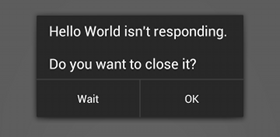
\includegraphics[width=0.6\textwidth]{img/anr-dialog.png}
 %   \caption{Race_Condition beim Shared Memory  \cite[vgl. ]{002}}
    \label{ANR Dialog}
  \end{centering}
\end{figure}
In diesem Beispiel greift Android in den Lebenszyklus der Aktivity ein, von der die zeitintensive Berechnung ausgeht und pausiert diese. Je nach Wunsch des Nutzers wird die Applikaiton dann in den Status \glqq Pausiert\grqq überführt, oder terminiert (siehe: onStoped() bzw. onDestroyed() im Lifecycle Diagramm) und vom Garbage Collector entsorgt (siehe hierzu Lebenszyklus einer Activity im nächsten Abschnitt). Die Zeit T innerhalb derer eine Applikation nicht auf Benutzereingaben reagiert und deren Ablauf der genannte Dialog erscheint ist für jedes Android Gerät konfigurierbar. Obwohl diese Eingreifmöglichkeit eine wichtige Funktion für die Kontrolle von Applikation durch den Nutzer darstellt, haben sich diverse Gerätehersteller mittlerweile entschieden die Zeit T sehr groß zu wählen, oder sogar den ANR-Dialog generell zu deaktivieren. In den Android Versionen ab Honeycomb führt das Blockieren einer Applikation bereits zur sofortigen Terminierung durch das Betriebssystem. Doch unabhängig vom ANR-Dialog bleibt der direkte Zusammenhang zwischen der Ansprechbarkeit einer Applikation und der Benutzbarkeit der Anwendung und dem Nutzererlebnis. Blockiert über zu lange Zeit eine Anwendung, so steigt damit auch die Unzufriedenheit des Nutzers über die Anwendung, besonders da er häufig die technischen Zusammenhänge, welche eine zeitintensive Verarbeitung durch aus rechtfertigen können, nicht kennt und gemäß der angesprochenen Designvorgaben auch nicht kennen muss.


\subsubsection{Komponentenmodell}
Bisher wurde die technische Ausführung von Android Applikationen auf der Betriebssystemebene erläutert. Für die einzelnen Konzepte der Nebenläufigkeit unter Android gilt es nun jedoch näher auf die Konzeption von Applikationen mittels klar definierten Komponenten selbst ein zu gehen, bevor im Kapitel 2 die einzelnen Konzepte an konkreten Implementierungsbeispielen verdeutlicht werden. Die folgende Abbildung zeigt die Basiskomponenten aus denen Anwendungen unter dem Android Betriebssystem bestehen:
\begin{figure}[H]
  \begin{centering}
    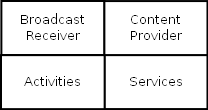
\includegraphics[width=0.6\textwidth]{img/Android_Komponent_Model.png}
 %   \caption{Race_Condition beim Shared Memory  \cite[vgl. ]{002}}
    \label{Android_Komponent_Model}
  \end{centering}
\end{figure}
\begin{itemize}
\item Broadcast Receiver erlauben die Registrierung von systemweiten oder applikationsinternen Events.
\item Content Provider repräsentieren Daten als relationalen Datensatz und ermöglichen den Zugriff über Applikationsgrenzen hinaus auf diese Daten.
\item Activities definieren das Verhalten von graphischen Benutzerschnittstellen
\item Services können zeitintensive Hintergrundberechnungen abbilden. 
\end{itemize}
Bei Services ist zu beachten, dass diese, wenn nicht anders definiert in dem Main Thread laufen, was jedoch für zeitintensive Verarbeitungen zu Problemen mit dem Benutzerinterface führen kann, wie in den folgenden Abschnitten näher beschrieben wird. Services dienen lediglich als mögliche Kapselung um Hintergrundverarbeitungen klarer vom Rest der Applikation zu trennen, sowie Verarbeitungen ohne aktives Benutzerinterface durchzuführen. Die Android Developper Dokumentation weist explizit darauf hin, keine zeitaufwändigen Verarbeitungen hier zu definieren wenn der Service im Main Thread läuft, da ansonsten die Gefahr besteht, dass der Main Thread und somit auch das Benutzerinterface blockiert. Dies gilt neben Services auch für die anderen Komponenten.

\subsubsection{Lebenszyklus einer Android Anwendung (Activity)}
Da sich diese Arbeit primär auf Applikationen mit Benutzerinterface konzentriert, macht es Sinn kurz auf den Lebenszyklus von Activities einzugehen der bereits in Kapitel \glqq Besonderheiten im Android Umfeld bezüglich des Thread Managements\grqq kurz aufgegriffen wurde.
Applikationen unter dem Android Betriebssystem unterscheiden sich in einigen Details deutlich von normalen Java Applikationen. Im Hinblick auf die nebenläufige Verarbeitung ist es daher von Bedeutung einen genaueren Blick auf den Lebenszyklus von Android Applikationen zu werfen. Die folgende Abbildung gibt einen Überblick über die Stati einer gestarteten Activity. Eine Objekt Instanz vom Typ android.os.Activity ist dabei der Einstiegspunkt in eine GUI-Applikation und wird vom Betriebssystem beim Start der Anwendung aufgerufen. Die einzelnen Statusübergänge, die in der Abbildung durch die jeweiligen Rückrufmethoden (onCreate(), onStart, onResume())symbolisiert werden,  sind für diese Arbeit weniger von Bedeutung. Interessanter sind die Abhängigkeiten zum Lebenszyklus des Prozesses, welcher für die Anwendung gestartet wurde, und damit die Frage nach der Lebensdauer von Threads. Die Abbildung zeigt deutlich zwei Szenarien in denen jeweils die Anwendung aus dem Sichtbarkeitsbereich des Nutzers entfernt wird (Übergang von onPaused() $\rightarrow$  onStop()). In dem ersten Szenario bleibt der Prozess nach dem Aufruf der onStop() Rückrufmethode bestehen. Das Android Betriebssystem behält damit die Reservierung des Adressraums im Speicher für diesen Prozess und ermöglicht ein schnelles Wiederaufrufen der Applikation, wenn der Nutzer dies wünscht (siehe in Abbildung Übergang von onStop() $\rightarrow$   onRestart()). Innerhalb des Prozesses definierte Nebenläufigkeit wird angehalten, d.h. die Ausführung aller Threads (auch des UI-Threads) wird unterbrochen. Die Threads selbst werden in den Status \glqq Wartend\grqq oder \glqq Schlafend\grqq überführt. Kehrt der Nutzer zu der Anwendung zurück, wird zunächst der UI-Thread wieder gestartet und in der Activity Instanz die Methode onResume() aufgerufen. Soll die nebenläufige Verarbeitung wieder gestartet werden, so empfiehlt es sich dies in der onResume() Methode zu implementieren.
\begin{figure}[H]
  \begin{centering}
    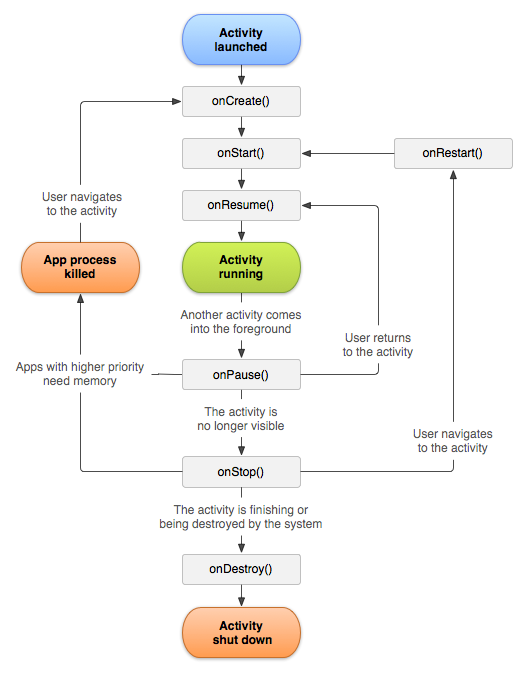
\includegraphics[width=0.9\textwidth]{img/activity_lifecycle.png}
 %   \caption{Race_Condition beim Shared Memory  \cite[vgl. ]{002}}
    \label{Activity_Lifecycle}
  \end{centering}
\end{figure}
Im zweiten Szenario wird der Adressraum dieses Prozesses für andere Anwendungen benötigt (siehe Abbildung onStop() $\rightarrow$  onCreate()). Das Betriebssystem terminiert in Folge dessen den Prozess und damit auch alle darin laufenden Threads. Für die Nebenläufigkeit auf Thread Ebene würde dies bedeuten, dass alle Threads zusammen mit dem Prozess mit terminiert werden. Kommt die Anwendung durch den Aufruf des Nutzers wieder in den Vordergrund, so wird zunächst wieder ein Prozess mit entsprechendem Adressraum vom Betriebssystem eingerichtet, der UI Thread neu erzeugt und nun in dem UI Thread die Activity neu instanziiert (dabei Aufruf onCreate()). Alle zuvor erzeugen sekundären Threads existieren nicht mehr. Die Verarbeitung im Hintergrund wurde unterbrochen und terminiert. Die Hintergrundverarbeitung lässt sich ggf. neu aus der onCreate Methode heraus neu starten.

\section{Anforderungen an Applikationen}
Abschließend zu dieser Einführung in die grundlegenden Konzepte zur Ausführung und den Bestandteilen von Android Applikationen, werden nun allgemeine Anforderungen an die Applikationen zusammengefasst, wie sie auch der Application Style Guide von Google vor gibt.
Applikationen für das Android Betriebssystem verfügen zum großen Teil über eine graphische Benutzeroberfläche, die wenigsten sind reine Hintergrund Programme. Darum liegt auch der Fokus der Applikationen auf deren Benutzbarkeit. Entsprechend ergeben sich auch besondere Anforderungen für die Entwicklung von Nebenläufigkeit. In Android Applikationen wird die Interaktion mit dem Benutzer über den Hauptthread (= UI- Thread), abgehandelt. Sind nun innerhalb einer Applikation zeitintensive Berechnungen oder andere Vorgänge definiert, so ist darauf zu achten, dass dadurch nicht der UI-Thread blockiert wird. Dieser soll stets bereitgehalten werden um mit dem Benutzer zu interagieren. Eine nebenläufige Verarbeitung ist also so zu definieren, dass sekundäre Threads vom UI Thread aus initialisiert und gestartet werden können und im Weiteren völlig losgelöst vom UI Thread operieren. Kommt es zum Nachrichtenaustausch zwischen dem UI Thread und den sekundären Threads (Datenaustausch) darf dies für den UI Thread keine zeitaufwändige Operation darstellen, diese Nachrichten zu verarbeiten. Weiter benötigt der Nutzer auch im Einzelfall Rückmeldung über den Bearbeitungsstand aus den sekundären Threads, sowie auch im Fehlerfall entsprechende Meldungen.

\section{Fokus und Eingrenzung}
In dieser Arbeit soll sich primär darauf konzentriert werden, wie asynchrone Parallelverarbeitung realisiert werden kann und welche Gefahren sich aus der Komplexität dieser Aufgabe ergeben können. Weiter ist die Fragestellung im Fokus, wie eine Fehlerbehandlung innerhalb asynchroner Parallelverarbeitung realisiert werden kann bzw. wie unterschiedliche Meldungen an den UI -Thread übertragen werden können. Um die Problemstellung der asynchronen Parallelverarbeitung für Andorid Plattformen greifbarer zu machen werden zwei Szenarien beschrieben in denen man bei der Implementierung die asynchronen Parallelverarbeitung sinnvoll demonstrieren kann:
\paragraph{Zugriff auf Web Ressourcen} 
In Android Applikationen ist es häufig nötig auf Web Ressourcen zu zu greifen. Bis jedoch die gesamte Ressource geladen ist, kann es u.U. je nach Verfügbarkeit des Netzwerks zu längeren Wartezeiten kommen. Arbeitet die Applikation nun streng sequentiell, so würde sie blockieren, bis die Ressourcen geladen sind und sich dann damit zurückmelden.
\paragraph{Zeitintensive Berechnungen}
Neben dem Zugriff auf Netzwerkressourcen können auch einzelne Berechnungen oder Suchfunktionen längere Zeit in Anspruch nehmen. Ebenso ist hier auf eine asynchrone Parallelverarbeitung zu achten, denn genauso wie in o.g. Szenario kann hier die Anwendung bei sequentieller Abarbeitung blockieren (also keine Benutzereingaben verarbeiten) und in Folge dessen durch das Betriebssystem terminiert werden. 
\newline
Die im Kapitel 2 aufgeführten Implementierungsbeispiele beziehen sich primär auf das zweite Szenario, um für Präsentationszwecke unabhängiger von Netzwerkeigenschaften zu sein.


\chapter{Asynchrone Parallelverarbeitung unter Android}
Für die Realisierung von asynchroner Parallelverarbeitung werden in diesem Kapitel drei Lösungsansätze entwickelt. Jeder dieser Ansätze versucht die asynchrone Verarbeitung im Hintergrund, losgelöst vom Hauptthread der Applikation zu realisieren. Als Beispiel für die im Hintergrund zu tätigende Verarbeitung steht eine rechenintensive und damit zeitaufwändige mathematische Operation. Ziel ist mit dieser Operation ausreichend Rechenauslastung zu erzeugen, sodass im Falle einer synchronen Abarbeitung die Applikation blockieren kann.

\section{Bolckierung der Ein-/Ausgabe durch zeitintensive Verarbeitung}
Dieser Abschnitt soll einen Einblick in das Verhalten von Applikationen unter dem Android Betriebssystem geben, wenn zeitintensive Berechnungen durchgeführt werden. Das Implementierungsbeispiel ist an das in Kapitel 1.9 beschriebene Szenario zu zeitintensiven lokalen Berechnungen angelehnt.
Die folgende Abbildung zeigt zwei Fenster einer Android Applikation mit je einem Knopf zum Start einer bestimmten zeitintensiven mathematischen Berechnung, deren Ergebnisse auf im jeweiligen Fenster angezeigt wird.
\begin{figure}[H]
  \begin{centering}
    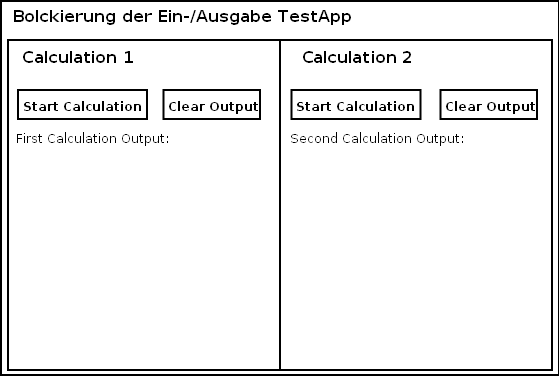
\includegraphics[width=0.9\textwidth]{img/BlockingIO_testApp_Mockup.png}
 %   \caption{Race_Condition beim Shared Memory  \cite[vgl. ]{002}}
    \label{BlockingIO_testApp_Mockup}
  \end{centering}
\end{figure}
Die mathematische Operation ist so gestaltet, dass sie im Komplexitätsgrad variabel einstellbar ist und somit auch die Verarbeitungszeit verlängert werden kann. Dabei handelt es sich um die Berechnung einer Quersumme aus einer sehr großen Primzahl. Die Ermittlung der Primzahl verlängert sich in Abhängigkeit zu der im Die mathematische Operation ist so gestaltet, dass sie im Komplexitätsgrad variabel einstellbar ist und somit auch die Verarbeitungszeit verlängert werden kann. Dabei handelt es sich um die Berechnung einer Quersumme aus einer sehr großen Primzahl. Die Ermittlung der Primzahl verlängert sich in Abhängigkeit zu der im Vorhinein definierten Mindestgröße der Primzahl (hier 1500Byte BigInteger):\newline\newline
\texttt{BigInteger veryBig = new BigInteger(1500, new Random());\newline
BigInteger randomPrimeNumber = veryBig.nextProbablePrime();\newline
int summe = 0;\newline\newline
while (0 != randomPrimeNumber.compareTo(BigInteger.ZERO))\newline 
\{ \newline
       // addiere die letzte ziffer der uebergebenen zahl zur summe \newline
       summe = summe + (randomPrimeNumber.mod(BigInteger.TEN)).intValue(); \newline\newline\newline
       // entferne die letzte ziffer der uebergebenen zahl \newline
       randomPrimeNumber = randomPrimeNumber.divide(BigInteger.TEN); \newline
       \} \newline
targetString.append(summe);\newline
}
Die Berechnung wird dabei angestoßen aus der Activity und allein innerhalb des UI Thread durchgeführt. In einem ersten Versuch wird die Komplexität nach und nach erhöht um zunehmend die Interaktion der Applikation mit dem Nutzer über die Benutzerschnittstelle zu blockieren. Nach einer bestimmten Blockierungszeit T ist zu beobachten, das der ANR Dialog des Betriebssystems erscheint und anbietet die Applikation zu beenden oder weiter zu warten. An dieser Stelle registriert das Betriebssystem, dass der UI-Thread als Haupt-Thread der Applikation für die Zeit T keine weitere Interaktion des Benutzers verarbeiten kann. Der Benutzer ist bis zu diesem Zeitpunkt nach Aktivierung der Berechnung nicht in der Lage die Applikation zu beenden oder zu wechseln. Daher schreitet nun das Betriebssystem ein, pausiert die Applikation und bietet dem Nutzer in einem ANR-Dialog an, die Applikation zu terminieren, oder weiter auf die Rückmeldung der Applikation zu warten.

\section{Parallelverarbeitung mit der Java Standard Edition (Java Concurrency)}
In diesem Beispiel wird nun versucht die zeitintensive Berechnung aus dem letzten Abschnitt, mittels der allgemeinen Mechanismen der Java Standard Edition in eine parallele Verarbeitung auszulagern. Damit soll das Blockieren der Anwendung verhindert werden. Hierzu wird die Berechnung in eine Klasse ausgelagert, die das Interface \texttt{java.lang.Runnable} implementiert. Diese kann darauf hin einem neuen Thread zur Ausführung übergeben werden. Der folgende Auszug aus dem Quellcode zeigt dabei den Konstruktor, sowie die \texttt{run()}- Methode der Klasse.\newline\newline\newline\newline\newline\newline
\texttt{
/$\ast\ast$\newline
$\ast$ The constructor.\newline
$\ast$ @param aView a view element.\newline
$\ast$ @param aCallbackHandler the Callback Handler for sending messages to ui-thread $\ast$/ %\newline
public RandomPrimeNumGenerator(final View aView, final Handler aCallbackHandler)\newline
\{ \newline
 Log.d(TAG,\grqq Call Constructor\grqq );\newline
 targetView = aView;\newline
 handler = aCallbackHandler;\newline
\} \newline
  @Override\newline
  public void run()\newline
  \{ \newline
     Log.d(TAG, \grqq Call run\grqq);\newline
       String result = startCalculation();\newline
       Message message = new Message();\newline
       Bundle bundle = new Bundle();\newline
       bundle.putCharArray(String.valueOf(targetView.getId()), result.toCharArray());\newline
       message.setData(bundle);\newline
       Log.d(TAG,\grqq Call handler\grqq );\newline
       handler.sendMessage(message);\newline
   \} \newline\newline
} \newline
Das hier verwendete Handler Objekt wird dem Konstruktor aus der Activity übergeben. Wird die durch den Konstruktor \texttt{RandomPrimeNumGenerator} erzeugte Runnableinstanz nun einem Thread Konstruktor übergeben und auf dieser Threadinstanz die \texttt{start()}- Methode Aufgerufen, so startet die Java Virtuelle Maschiene einen neuen Thread, der die zeitintensive Berechnungen ausführt. Der folgende Codeabschnitt ist in der Activity defininiert. Es wird somit aus dem Main Thread heraus ein neuer Thread erzeugt.\newline\newline\newline
\texttt{
private final Handler handler = new Handler();\newline\newline
public void initCalculation(View aView)\newline
  \{ \newline
     RandomPrimeNumGenerator runnable =
        new RandomPrimeNumGenerator(aView, handler);\newline\newline  
     Thread newThread = new Thread(runnable);\newline
     newThread.start();\newline
  \} \newline
} \newline

\glqq Wartend\grqq








\section{Erkennung und Interpretation von Gesten sowie Steuerung jeweiliger Funktionalität durch Gesten}
Für die Erkennung von Gesten bietet das Android SDK die Schnittstelle OnTouchListener an. Darin lässt sich die Methode\newline
   \centerline{ \texttt{boolean onTouch(View zoomView, MotionEvent anEvent)\{...\}}}\newline
überschreiben. Über den Parameter anEvent vom Typ MotionEvent können unterschiedliche Berührungsgesten erkannt werden. Die Methode OnTouchListener wird in Abhängigkeit von bestimmten Ereignissen aufgerufen. Hierzu ist zu einer View-Instanz die konkrete Implementierung des OnTouchListener Interfaces zu adressieren:\newline \centerline{\texttt{viewInstance.setOnTouchListener(touchListenerImpl);}}\newline
Wenn der Touchsensor eine Berührung registriert, wird für das jeweilige Layout geprüft, welche darin enthaltenen Views die Methoden des OnTouchListeners überschreiben und das Event an die jeweilige Implementierung weitergeleitet. Des Weiteren ist dem Objekt vom Typ MotionEvent zu entnehmen, um welche Art von Berührung es sich handelt.
Je nach Art und Weise der Berührung liefert die Maskierung der zur Event Aktion\newline
\centerline{\texttt{anEvent.getActionMasked()}}\newline\newline
ein Ergebnis, welches durch ein Element der Menge aus den folgenden Konstanten beschrieben wird:\newline
Menge M\newline
\{\newline\texttt{
   int ACTION\_DOWN = 0;\newline
   int ACTION\_UP = 1;\newline
   int ACTION\_MOVE = 2;\newline
   int ACTION\_CANCEL = 3;\newline
   int ACTION\_OUTSIDE = 4;\newline
   int ACTION\_POINTER\_DOWN = 5;\newline
   int ACTION\_POINTER\_UP = 6;\newline
   int ACTION\_HOVER\_MOVE = 7;\newline
   int ACTION\_SCROLL = 8;\newline
   int ACTION\_HOVER\_ENTER = 9;\newline
   int ACTION\_HOVER\_EXIT = 10;\newline}
\}\newline \newline
Für die Interpretation der Gesten und weiter die Steuerung exemplarischer Funktionalitäten wie Zoom oder Drag gilt dann:\newline\newline
ACTION\_DOWN: Der Touchsensor registriert eine Berührung in einem in sich geschlossenen Bereich.\newline
Beispiel: Die Fingerkuppe eines Nutzers berührt den Touchscreen. Die Koordinaten erhält der Entwickler durch das Auslesen des Event-Parameters. Über die Methoden\newline
\centerline{\texttt{anEvent.getX()} und}  \newline
\centerline{\texttt{anEvent.getY()}}\newline
können die Koordinaten ausgelesen werden, auf denen sich ein Finger auf dem Touchbildschirm befindet. Diese Methoden geben im Fall von mehrerer Berührungen (z.B. mehrere Finger) immer die Koordinaten des ersten Berührungspunktes an.\newline\newline
ACTION\_UP: Der Touchsensor registriert das Aufheben einer ursprünglich registrierten Berührung. Dies setzt zuvor die Registrierung einer ACTION\_DOWN voraus.\newline\newline
ACTION\_POINTER\_DOWN:
Der Touchsensor registriert eine zweite Berührung (zweiter Finger). Die Koordinaten der zweiten Berührung, sowie auch im Falle weiterer Berührungspunkte, lassen sich aus dem Event entsprechend der Reihenfolge der Berührung ermitteln:
\centerline{\texttt{anEvent.getX(0..n);}}\newline
\centerline{\texttt{anEvent.getY(0..n);}}\newline
Dies entspricht der Berührung mit dem ersten bis N-ten Finger. Für die Funktionalität Zoom ist es notwendig, die initiale Distanz zwischen den zwei Berührungspunkten zu ermitteln und temporär vorzuhalten.\newline\newline
ACTION\_MOVE: Der Touchsensor registriert eine Bewegung weg vom ursprünglich registrierten Berührungspunkt, dessen Ermittlung diesem Event vorausgeht. Um die o.g. Funktionalitäten zu realisieren, wird für die Ein-Finger-Geste "Drag" der Richtungsvektor bei einer Bewegung auf dem Touchbildschirm ermittelt, indem vom initialen Berührungsspunkt bis zur aktuellen Position des Fingers die Differenz in x wie in y Richtung errechnet wird.


\section{Gestengesteuertes Vergrößern und Verkleinern sowie Veränderung des Fokus für Darstellungsobjekte vom Typ ImageView}
Ian F. Darwin liefert mit seinem Kochbuch für die Android Entwicklung zu der Zoomfunktionalität folgenden Ansatz: \newline
\texttt{// Remember some things for zooming \newline
PointF start = new PointF();\newline\newline
ImageView view = (ImageView) v;\newline
// make the image scalable as a matrix \newline
view.setScaleType(ImageView.ScaleType.MATRIX);\newline
...\newline
switch (event.getAction() \& MotionEvent.ACTION\_MASK) \{ \newline
case MotionEvent.ACTION\_DOWN: //first finger down only\newline
start.set(event.getX(), event.getY());\newline
break;\newline
...\newline
case MotionEvent.ACTION\_MOVE:\newline
if (mode == DRAG)\newline
matrix.postTranslate(event.getX() - start.x, event.getY() - start.y);\newline
\newline
else if (mode == ZOOM)\newline
matrix.postScale(scale, scale, mid.x, mid.y);\newline
\newline
// Perform the transformation\newline
view.setImageMatrix(matrix);\newline
\} \newline 
}\cite[S. 234-237.]{003}\newline
Diese Auszüge aus Darwins Kochbuch zur Andorid Entwicklung zeigen schematisch die dynamische Skalierung einer ImageView in Abhängigkeit der erkannten Gesten mit Hilfe einer speziell für diesen Objekttyp anpassbaren Matrix. Die Matrix lässt sich direkt aus einer Objektinstanz vom Typ ImageView holen und mittels der Methoden
\begin{itemize}
\item \texttt{postTranslate()} und
\item \texttt{postScale()}
\end{itemize}
verarbeiten. Dabei ist zu beachten, dass die Matrix nicht direkt verändert werden darf, sondern nur deren Kopie. Der Richtungsvektor für die neue Fokussierung und damit Transformation der Matix errechnet sich aus der Differenz der aktuellen Koordinaten zu den Anfangskoordinaten und wird zur Transformation der Matrix entsprechend übergeben:\newline
\centerline{ \texttt{ matrix.postTranslate(event.getX() - start.x,}} \newline \centerline{ \texttt{ event.getY() - start.y) }}\newline \newline
Im Fall von mehreren registrierten Berührungen, wie z.B. bei der Pinch-Open-Geste für die Ansteuerung einer Zoom-Funktionalität, muss zunächst die Anfangsdistanz zwischen den Berührungspunkten auf dem Touchbildschirm ermittelt werden. In einem Koordinatensystem aus zwei Dimensionen (x|y) wird die Länge einer Strecke von P1(xp1|yp1) und P2(xp2|yp2) wie folgt berechnet:
\centerline{$\sqrt{(x_{0}-x_{1})^{2}+(y_{0}-y_{1})^{2}}$ }\newline\newline
In Darwins Implementierung ist dies in der Methode \texttt{spacing()} realisiert. Weiter ist über das gesamte ACTION\_MOVE Event hinweg, die neue Distanz der Berührungspunkte zu berechnen und mit der initialen Distanz in ein Verhältnis zu setzen. Der Quotient aus
\centerline{$ ScaleFaktor = \dfrac{dist_{new}}{dist_{old}}$} \newline\newline
ergibt den Faktor für die Skalierung der ImageView. Die ImageView wird daraufhin entsprechend relativ zu der Positionsänderung der Berührungspunkte neu skaliert.\newline
\centerline{ \texttt{ matrix.postScale(scale, scale, mid.x, mid.y);}} \newline\newline
Darwins Vorgehensweise stellt eine komfortable und einfache Möglichkeit dar, eine ImageView Instanz dynamisch zu skalieren oder den Fokus der Darstellung zu verändern. Jedoch bezieht sich die Lösung allein auf Darstellungselemente vom Typ ImageView, wohingegen die Superklasse View, die durch ImageView erweitert wird, es nicht vorsieht die Matrix zur Skalierung und Positionierung der View direkt zu verändern. Damit ist Darwins Lösung allein für Darstellungsobjekte vom Typ ImageView geeignet.

\section{Abstraktion gestengesteuerter Funktionalitäten zum Skalieren und Fokussieren von Darstellungselementen}
Dieser Abschnitt beschäftigt sich mit der Frage, inwieweit sich der Ansatz von Darwin generalisieren lässt und somit unabhängiger vom Typ des Darstellungsobjektes wird. Kann hierzu eine Lösung gefunden werden, so ist weitergehend zu diskutieren, inwieweit diese für andere Android App Projekte verfügbar gemacht werden kann.

\subsection{Generalisierung der Funktionalitäten zum Skalieren und Fokussieren von Darstellungselementen}
Die skizzierte Implementierung nach I.F. Darwin im letzten Abschnitt zeigt zwar, wie ein bestimmtes Darstellungselement in Abhängigkeit von bestimmten Gesten skaliert, jedoch gilt diese Lösung nicht für andere Darstellungselemente. Ein generischer Ansatz müsste die Skalierung und Fokussierung für alle Darstellungselemente leisten, mindestens jedoch für alle Elemente, die vom Typ android.view.View ableiten.\newline
Der im Folgenden skizzierte Prototyp soll Darwins Ansatz um eine dynamische Anzahl von Darstellungselementen mit der Kompatibilität zu unterschiedlichen Darstellungstypen erweitern.
Dieser Projektarbeit liegt eine prototypische Implementierung bei (Klasse \texttt{Touch.java}), in der das Skalieren und Fokussieren von Darstellungselementen für allgemein alle Objekte ermöglicht wird, die vom Typ \texttt{android.view.View} ableiten (z.B. \texttt{TextView extends View}). Ein entsprechender Algorithmus könnte damit die Funktionalität zur Skalierung und Fokussierung applikationsübergreifend generalisieren. 
Für die Skalierung eines Darstellungsobjektes vom Typ View bietet die Android API folgende Methoden an:
\begin{itemize}
\item \texttt{setScaleX()}
\item \texttt{setScaleY()}
\end{itemize}
und für die Veränderung des Fokus auf die View:
\begin{itemize}
\item \texttt{setTranslationX()}
\item \texttt{setTranslationY()}
\end{itemize}
Ein dabei auftretendes Problem sind unerwünschte Seiteneffekte bei der Verwendung des Listeners zur Registrierung von Berührungen und Bewegungen. Dieser Listener kann einer View zugeordnet werden:
\centerline{\texttt{viewInstance.setOnTouchListener(touchListenerInstance)}}\newline \newline
Wird jedoch dieselbe View-Instanz innerhalb der TouchListener-Implementierung neu skaliert, kommt es auf Grund der angestoßenen Zoom-Funktionalität zu einem flackernden Übergang von der ursprünglichen Skalierung in die neue Skalierung. Dies liegt daran, dass das Koordinatensystem der View durch die Skalierung unmittelbar selbst verändert wird. Stellt diese View jedoch auch das Koordinatensystem für die Gestenerkennung, (\texttt{viewInstance.setOnTouchListener(...)}), so wird die Berechnung des Zoomfaktors gestört.
 \newline
Die View, welche durch den Zoom neu skaliert wird, darf also im Falle einer gestengetriebenen Zoom-Funktionalität nie die Bemessungsgrundlage (Koordinaten) für die Berechnung des Skalierungsfaktors sein. Alternativ kann die sogenannte Parent-View der zu skalierenden View-Instanz als Bemessungsgrundlage herangezogen werden, wie es die folgende Abbildung zeigt: \newline
\begin{figure}[H]
  \begin{centering}
    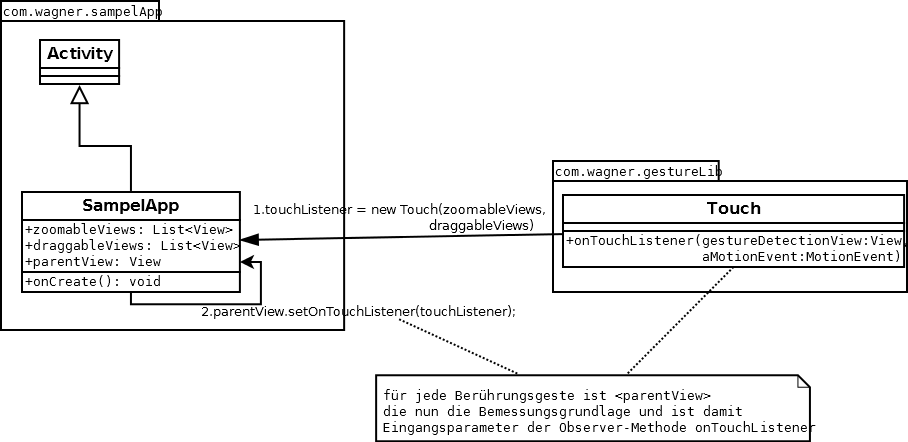
\includegraphics[width=0.8\textwidth]{img/touchFragments.png}
    \caption{Konzeption eines generischen Touchlisteners}
    \label{callingTouchListener}
  \end{centering}
\end{figure} Die Parent-View ist in der Baumstruktur des Layouts einer View- Instanz übergeordnet. 

\subsection{Ausblick zur Integration der generischen Implementierung zu gestengesteuerten Funktionalitäten}
Der letzte Abschnitt hat gezeigt, wie gestengesteuerte Funktionalitäten zum Skalieren und Fokussieren von Darstellungselementen, allgemein für unterschiedliche Darstellungstypen definiert werden können. Dieser Abschnitt gibt einen Ausblick, wie der entworfene Ansatz aus dem letzten Kapitel allgemein für Android Applikationsprojekte angeboten werden kann.\newline
In Android Projekten lassen sich wie auch in anderen Java Projekten zusätzliche Bibliotheken in Form von .jar - Archiv Dateien einbinden. Grundsätzlich ist es möglich diese Bibliotheken manuell in die jeweilige Entwicklungsumgebung einzufügen. Sollten jedoch unterschiedliche Versionen zu den jeweiligen Android APIs unterschieden werden sind bestimmte Werkzeuge zur Versionverwaltung und dem übersichtlichen Management von Abhängigkeiten zu empfehlen. Auch wenn Tests zu Funktionalitäten der Bibliothek vor dem Erzeugen des .jar - Archives durchlaufen werden müssen, sollte dies automatisiert sein. Hierzu gibt es unterschiedliche Werkzeuge, die sich für das Auflösen von Abhängigkeiten sowie das finale Bauen der Applikation anbieten. Exemplarisch bietet sich hier das Build Werkzeug \glqq Maven\grqq mit dem Android Plugin an. Der im letzten Kapitel entworfene Ansatz lässt sich damit in eine eigenständige Bibliothek auslagern, um diesen in unterschiedlichen Android-Applikationsprojekten zu nutzen.

\section{Fazit}
Eingangs stand die Frage im Raum, wie den Einstiegshürden in der Android-Entwicklung sowie dem Problem des Code-Copy entgegen gewirkt werden kann. Anhand der Entwicklung von gestengesteuerter Funktionalität (speziell hier Zoom und Drag) ist verdeutlicht worden, welche Schwierigkeiten auf Einsteiger in der Android Entwicklung warten. Gleichzeitig wird mit der Implementierung nach Darwin (Kapitel 3.3) deutlich, welche Mengen an komplexem Sourcecode zu gestengesteuerter  Funktionalität (siehe Implementierung nach F.Darwin Kapitel 3.3) in Applikationsprojekte integriert werden müsste, um grundlegendes Verhalten zu definieren. Der in diesem Projekt geschaffene Ansatz zur Generalisierung von gestengesteuerter Funktionalität bietet die Möglichkeit den dahinterstehenden Programmcode zu zentralisieren, also Code Copy vorzubeugen und gleichzeitig die Android App-Entwicklung zu vereinfachen.
Für weitere gestengesteuerte Funktionalitäten kann ähnlich verfahren werden, vorausgesetzt es kann ein geeigneter Abstraktionsgrad gefunden werden, wie er hier für die Skalierung und Fokussierung definiert ist.

\bibliography{Praxisprojekt}{}
\bibliographystyle{jureco} %% jurabib, jureco, jurunsrt, 
%% \printindex

\appendix

\chapter*{Anhang}
 \lstinputlisting
    [caption={Die Klasse Touch.java}
       \label{lst:javaclass},
       captionpos=t,language=JAVA]
 {listings/Touch.java}
\addcontentsline{toc}{chapter}{Anhang}
\chapter{Erklärung}

Ich versichere, die von mir vorgelegte Arbeit selbständig verfasst zu
haben. Alle Stellen, die wörtlich oder sinngemäß aus veröffentlichten
oder nicht veröffentlichten Arbeiten anderer entnommen sind, habe ich
als entnommen kenntlich gemacht. Sämtliche Quellen und Hilfsmittel,
die ich für die Arbeit benutzt habe, sind angegeben. Die Arbeit hat
mit gleichem Inhalt bzw. in wesentlichen Teilen noch keiner anderen
Prüfungsbehörde vorgelegen.

\bigskip

Gummersbach, den \today

\bigskip

\bigskip

\bigskip

\bigskip

\bigskip

\bigskip

(Unterschrift)

\end{document}

%% end of file
